\documentclass[../main.tex]{subfiles}

\graphicspath{{\subfix{../imgs/}}}

\begin{document}

\section{Task 3.5}

Implement a model that demonstrates a system design that transfer data at the TLM level refined to BCAM level. Use the \texttt{sc\_fifo} to model communication at the TLM level and refine it to BCAM using adapters. As inspiration study the example project \textbf{SmartPitchDetector}. Here a master sends data to a slave using a \texttt{sc\_fifo} and an adpater that converts to the bus cycle accurate interface on the receiving slave. Use the model from task 3.4 for the interface at the Avalon-ST sink interface for the slave as illustrated below.

\begin{figure}[h]
    \centering
    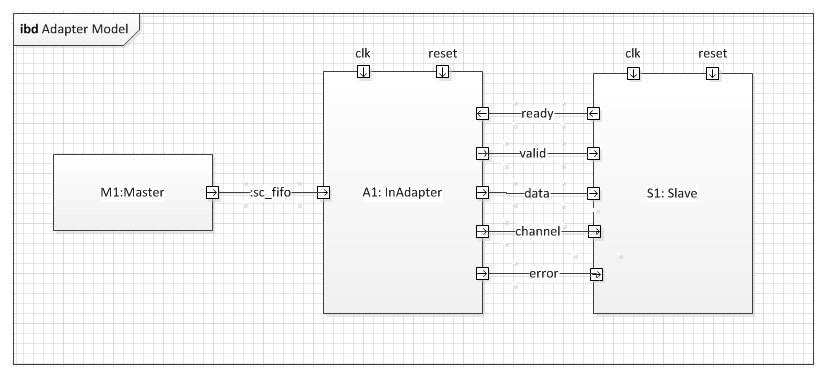
\includegraphics[width=0.9\textwidth]{task3_5.png}
    \caption{Task 3.5 overview.}
\end{figure}

\subsection*{Solution}

We started by designing a master module from $sc\_module$ that transmits data into a fifo. For this purpose, it just transmits an 8-bit number.

\begin{myminted}{/inc/Master.cpp}
#include "Master.hpp"
Master::Master(sc_module_name name) : sc_module(name)
{
	SC_THREAD(generateDataForAdapter);
}
void Master::generateDataForAdapter() {
	sc_uint<8> data = 0;
	while (true){
		wait(MASTER_OUTPUT_PERIOD, MASTER_OUTPUT_PERIOD_UNIT);
		out_fifo->write(data++);	
	}
}
\end{myminted}

The fifo is then connected to an adapter module, that converts the data from the fifo to the BCAM interface. The adapter module is implemented as follows:

\begin{myminted}{/inc/InAdapter.hpp}
class InAdapter : public sc_module, public sc_fifo_out_if<T> {
public:
	sc_in_clk clock;
	sc_in<sc_logic> ready, reset;
	sc_out <sc_logic> valid;
	sc_out<CHANNEL_BITS> channel;
	sc_out<ERROR_BITS> error;
	sc_out<DATA_BITS> data;

	InAdapter(sc_module_name name) : sc_module(name) {};

	void write(const T& value) {
		if (reset.read() == SC_LOGIC_0) {

			while (ready.read() == SC_LOGIC_0) {
				wait(clock.posedge_event());
			}
			wait(clock.posedge_event());

			data.write(value);
			channel.write(0);
			error.write(0);
			valid.write(SC_LOGIC_1);

			wait(clock.posedge_event());
			valid.write(SC_LOGIC_0);
		} else {
			wait(clock.posedge_event());
		}
	}
private:
	bool nb_write(const T& value) {
		SC_REPORT_FATAL("/InAdapter", "Called nb_write()");
		return false;
	}
	int num_free() const {
		SC_REPORT_FATAL("/InAdapter", "Called num_free()");
		return -1;
	}
	const sc_event& data_read_event() const {
		SC_REPORT_FATAL("/InAdapter", "Called data_read_event()");
		static sc_event dummy_event;
		return dummy_event;
	}
};
\end{myminted}

\newpage

The adapter module inherits $sc\_module$ and $sc\_fifo\_out\_if$. The write method is implemented to convert the data from the fifo to the BCAM interface. 
When the reset signal is low, the adapter waits for a ready signal from the slave. When the ready signal is set to high by the slave, the adapter sets the valid signal to high and waits one cycle before transmitting the data to the slave.

\begin{myminted}{/inc/slave.cpp}
#include "Slave.hpp"

Slave::Slave(sc_module_name name)
{
	SC_METHOD(receive);
	sensitive << clock.pos();
}
void Slave::receive()
{
	if (reset.read() == SC_LOGIC_0) {
		if (valid.read() == SC_LOGIC_1) {
			ready.write(SC_LOGIC_0);
		} else {
			ready.write(SC_LOGIC_1);
		}
	}
}
\end{myminted}
While reset is low, if the valid signal from the adapter is high, the ready signal is set to low. Otherwise it is set to high.

In the figure we can see the trace from the simulation. 

\begin{figure}[h]
    \centering
    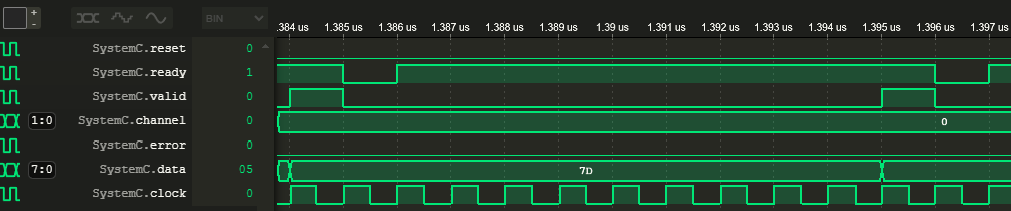
\includegraphics[width=1.0\textwidth]{trace_3_5.png}
    \caption{Trace from the simulation of task 3.5}
\end{figure}


\end{document}